\documentclass{mcmthesis}
\mcmsetup{CTeX = false,   % 使用 CTeX 套装时,设置为 true
        tcn = 2108321, problem = C,
        sheet = true, titleinsheet = true, keywordsinsheet = true,
        titlepage = false, abstract = false}
\usepackage{palatino}
\usepackage{lipsum}
\usepackage{float}
\usepackage{geometry}
%===============设置正文和数学字体=============================
%有些字体需要安装一些字体文件,注意辨别。
%我参照 MCM论文集的字体 使用如下宏包来定制字体。

\usepackage{graphicx}

\usepackage{subfigure}
%设置段落之间的距离,若不需要删除或者注释掉即可。
\setlength\parskip{.5\baselineskip}
\newtheorem{definition}{Definition}[section]
%\def\abstractname{Summary}%可修改摘要名称
\usepackage{url}
\usepackage{indentfirst}
\setlength{\parindent}{2em}
\usepackage{siunitx}
\usepackage{chngpage}
\usepackage{array}
\usepackage{booktabs}
\usepackage{threeparttable}
\usepackage{longtable}
\usepackage[numbers,sort&compress]{natbib}
\usepackage{amsmath}
\numberwithin{figure}{section}
\numberwithin{table}{section}
%%% 实现参考文献标号在右上角
\newcommand{\upcite}[1]{\textsuperscript{\textsuperscript{\cite{#1}}}}
%然后引用的时候使用\upcite{}的格式(一般的正常引用格式为\cite{})



\usepackage{titletoc}
\titlecontents{section}[3cm]{\bf \large}{\contentslabel{2.8em}}{}{%
\titlerule*[0.5pc]{$\cdot$}\contentspage}%
\titlecontents{subsection}[4cm]{\normalsize}{\contentslabel{2.5em}}{}{%
\titlerule*[0.5pc]{$\cdot$}\contentspage}%
\titlecontents{subsubsection}[5.3cm]{\normalsize}{\contentslabel{3.0em}}{}{%
\titlerule*[0.5pc]{$\cdot$}\contentspage}%



\title{\large The Prediction to the Migration of Scottish Herring and Mackerel }
\author{}
\date{\today}
\geometry{left=2.5cm,right=2.5cm}

\begin{document}



\begin{abstract}
  This paper establishes a model for the spread of Vespa mandarinia over time and a priority assessment model for eyewitness reports. By analyzing the notes, pictures, and sighting locations provided by the eyewitnesses, the multimodal classification model established in this paper is able to lead to prioritizinginvestigation of the reports most likely to be positive sightings.
  
  For the spread of Vespa mandarinia over time , this paper analyzed the distribution of honey bee hives, vegetation cover, hornet habits, and rated the risk for each county in Washington. This paper then inferred three possible spread routes of hornet and a key area for hornets. For the priority assessment model of eyewitness reports, this paper uses three sub-classification models to obtain the final multimodal classification model, which specifically includes a risk assessment model based on the location of the sighting, a note classification model based on Naive Bayes, and a picture classification model based on EfficientNet. In this paper, the original data are firstly preprocessed with formatting, data enhancement, sample equalization,  training set slicing, and then the three sub-models are trained independently. Finally the hyperparameters of model fusion are analyzed for sensitivity. Considering the existence of many unlabeled samples, this paper uses a semi-supervised approach to train the models. Considering the dynamic expansion of samples, this paper suggests using batch learning to update the model when the number of new samples reaches 400.
  
  This paper prioritizes the Unprocessed and Unverified labeled samples and lists the top eight samples in terms of likelihood of Vespa mandarinia occurrence. This paper summarizes the advantages and disadvantages of the model, and puts forward the future improvement work.
  
\begin{keywords}
EfficientNet; Naive Bayes; Semi-supervision; Batch Learning  

\end{keywords}
\end{abstract}
\maketitle
\pagestyle{empty}
\newpage                                                          %
%==================================================================
%====================生=成=目=录===================================
\begin{adjustwidth}{-1cm}{0cm}

\setcounter{tocdepth}{3}
\thispagestyle{empty}
\tableofcontents                                                  %

\end{adjustwidth}


\newpage

\pagestyle{fancy}

\setcounter{page}{1}
\section{Introduction}
\subsection{Background}

The Asian giant hornet is the largest and most cruel hornet in the world. It looks like a AA battery with wings and armor. It also has a huge stinger and eagers to bite off the bee’s head and sting people. The name "killer bumblebee" comes from this giant insect that can kill the entire bee colony, and the deaths of dozens of people each year are also related to them.

What makes people worried is that North American bees do not know how to fight back Asian giant hornet like Asian bees. Asian bees will use a strategy called "hotball" to kill Asian hornet. This strategy means that Asian honeybees will swarm on a Asian giant hornet that is much larger than them and begin to vibrate their small bodies, producing enough heat to effectively "cook" the hornet from within, thereby killing it. Experts worry that Vespa mandarinia hornet may have catastrophic consequences for European bees in North America. The number of European honeybees in North America was reduced due to pesticides and many other factors. Now such a huge enemy has been added.

Considering the huge threat of the Asian giant Hornet, it is particularly important for the Washington Department of Agriculture to take precise measures to eliminate it. Therefore, the Washington State Department of Agriculture said in a statement: “The most likely time to catch the Asian giant Hornet is from July to October. This is when the colony is established and the workers are foraging. If you want to trap the queen, the earliest the trap can be hung in April, but because the number of queens is significantly less than the workers, the possibility of catching the queen is very small." These researchers are working with the Washington State Department of Agriculture, beekeepers and the public to find and study these giant hornets, and prevent its spread.

This article discusses the spread of Asian giant hornets over time and hopes to help the Washington Department of Agriculture deal with more urgent reports by predicting the probability of this sighting being a Vespa mandarinia based on pictures, notes, sighting locations, time and other information reported by witnesses.


\subsection{Problem Analysis}

% 问题一:建立一个数学模型,以确定这两种鱼类在未来50年内最有可能出现的位置,假设水温变化足以导致种群移动。

% 问题二:根据海水温度变化,使用您的模型预测最佳情况和最坏情况,到时这些小渔业公司因距离鱼群太远将无法收获。

% 问题三:根据你的预测分析,这些小型渔业公司是否应该改变他们的经营?

% a、如果是,请使用您的模型来确定和评估对小型渔业公司具有实际和经济吸引力的战略。你的策略应该考虑但不限于现实的选择,包括:

%  -将渔业公司的部分或全部资产从苏格兰港口的当前位置转移到更靠近两个鱼类种群移动的位置;

% -使用一定比例的小型渔船,可以在没有陆地的情况下作业一段时间,同时仍然确保渔获物的新鲜度和高质量。

% b、如果您的团队拒绝任何更改的需要,请根据您的建模结果证明您拒绝的原因,因为它们与您的团队所做的假设有关。

% 问题四:如果某一比例的渔业进入另一个国家的领海(海洋),请使用您的模型来说明您的方案受到的影响。

% 问题五:除了你的技术报告外,为相关组织准备一到两页的文章,以帮助渔民了解问题的严重性,以及你提出的解决方案将如何改善他们未来的商业前景。
\begin{itemize}
  \item \textbf{Address and discuss whether or not the spread of this pest over time can be predicted,and with what level of precision.}
  
First, we analyze the living habits and determine the suitable living environment of Vespa mandarinia. Then we comprehensively consider the distribution of bee hives in each county in Washington State, vegetation coverage, traffic topography and other factors, and score the basic situation of each county in Washington State. Combining these objective factors and a small amount of wasp sighting samples, we can easily analyze the distribution of this pest over time. Considering that the number of positive samples is less than 20 and the distribution area is very cramped, we can roughly divide the key areas of Asian giant hornet distribution and the possible migration routes over time. The accuracy of the model can be measured by analyzing the number of positive samples that fall in the area.
  
  \item \textbf{Most reported sightings mistake other hornets for the Vespa mandarinia. Use only the data set file provided, and (possibly) the image files provided, to create, analyze, and discuss a model that predicts the likelihood of a mistaken classification.}

Most of the samples were mistaken as Vespa mandarinia by eyewitnesses, and these samples wereted a lot of staff confirmation time. Therefore, it is necessary to determine the priority of the report through the pictures, notes, sighting location, time and other information provided in the eyewitness report. For this multi-modal binary classification model, we obtain the report priority through the weighted fusion of the three sub-classification models. Specifically, we use EfficientNet to complete the two classification of images, use Naive Bayes to complete the two classification of notes, and use the risk assessment model to complete the two classification of sighting locations. 
  
First, we format the original data, clean the data, and then segment the data according to different sub-model requirements. In addition, it is necessary to appropriately expand the positive samples to solve the problem of sample imbalance. For the picture classification model, data enhancement is also needed to enhance the robustness of the model. For pictures with more unprocessed and unverified tags, a semi-supervised learning method is used to complete the two classification in the iterative process. Finally, we sum up the scores of the three sub-models as the final score.


  \item \textbf{Use your model to discuss how your classification analyses leads to prioritizing investigation of the reports most likely to be positive sightings.}

The output of our model represents the priority level of the report. If it is higher than a certain threshold, the staff should give priority to it. The score priorities of the three sub-models are different. The image classification model has the highest priority, the sighting location risk assessment model is the second, and the comment classification model has the lowest priority.

  \item \textbf{Address how you could update your model given additional new reports over time, and how often the updates should occur.}
  
The number of reports that can be used for training will gradually increase over time. In order to ensure that the performance of the model can continue to improve, we need to update the model in the manner of batch learning when the number of new samples reaches 400, about 20 days.

  \item \textbf{Using your model, what would constitute evidence that the pest has been eradicated in Washington State?}

We use our model to evaluate the priority of reports with unprocessed and unverified labels. If all priority of reports are lower than the default threshold and combining the living habits of the Vespa mandarinia, we can infer that the Asian giant hornet has been eradicated in Washington State with the statistical law.

\end{itemize}


\section{Assumptions and Symbols Definitions}
\subsection{Assumptions}

\begin{itemize}
\item It is assumed that that the data is true and valid and the source is reliable.

\item It is assumed that the migration of Vespa mandarinia over time is completely determined by its living habits and environment.

\item It is assumed that every position of Asian giant hornet can be immediately discovered by witnesses.


\item It is assumed that the manually constructed positive sample and the real sample have the same distribution.


\item It is assumed that the fusion model can always break through the data bias of a single model.


\end{itemize}


\subsection{Symbols Definitions}

\begin{center}
\begin{longtable}{p{.1\textwidth}p{.8\textwidth}m{.4\textwidth}}
\caption{The List of Notation}\\
\hline
Symbol& Meaning \\
\hline

$A$      & A eyewitness location-based Risk assessment model
                                                         \\
$B$      & A Plain Bayesian-based Notes Classification Model
                                                          \\
$C$     & A EfficientNet-based Picture Classification Model
                                                        \\
$D$       & The fusion model of the above three single models                                                       \\
$S_i$      & The priority score of model i, the value range is $0 \sim 1$, 1 corresponds to the highest priority
                                                            \\
$(x_0,y_0)$       & The center coordinate of the key area
                                 \\
$r_0$       & The radius of the key area
                                         \\
$(x,y)$       & The sighting location, x represents latitude and y represents longitude
\\
$r$       & The distance from the sighting location to the center of key area \\
$F_1$       & The risk score based on the distance from the key area, the value range is $0 \sim 1$, 1 corresponds to the highest risk level \\
$F_2$      &  The risk score based on the number of bee hives and vegetation coverage, the value range is $0 \sim 1$, 1 corresponds to the highest risk level
\\
$\gamma$      &  The weight of $F_1$ in model A, the range is $0 \sim 1$

\\
$\alpha$       & The weight of model A in model D, the range is $0 \sim 1$

\\
$\beta$       & The weight of model B in model D, the range is $0 \sim 1$
\\
$1-\alpha-\beta$       & The weight of model C in model D, the range is $0 \sim 1$
\\
                                                        \\ \hline

 \end{longtable}
 \end{center}


\section{Establishment and Solution of Model}
\subsection{Modeling changes in the distribution of Asian hornets}

The life cycle of an Asian giant hornet begins with a queen’s nest building after overwintering. During this period, the queen develops a nest, collects and eats arthropods and sap, and prepares to lay eggs. The colony begins in summer, the queen takes care of her cubs, and worker ants finally begin to appear. Once the queen has produced enough workers, the responsibility of predation is completely transferred to the workers, and the queen stays in the nest to continue laying eggs.


In order to estimate the risk of Asian giant hornet to Washington, we have carried out a risk rating for each county in Washington. The reference standards are as follows: 
\begin{enumerate}
  \item Winter climate suitability
  \item Whether the habitat is suitable for Asian giant hornet colonization nests (This is based on the dense forest biomass)
  \item The hive density of the counties
  \item The path (main port or freight hub) that may introduce Asian Hornet
\end{enumerate}

Because the prey objects of Asian giant hornet are mainly honeybees, and the nesting and reproduction of Asian giant hornet are inseparable from trees and vegetation, we recommend that the Washington government pay more attention to counties with a large number of hives, extensive vegetation coverage, and convenient transportation. We consulted relevant information \cite{REF1} and sorted out the number of hives and vegetation coverage in each county in Washington. The following figure shows the corresponding data:



\begin{figure}[H]
  \centering{
  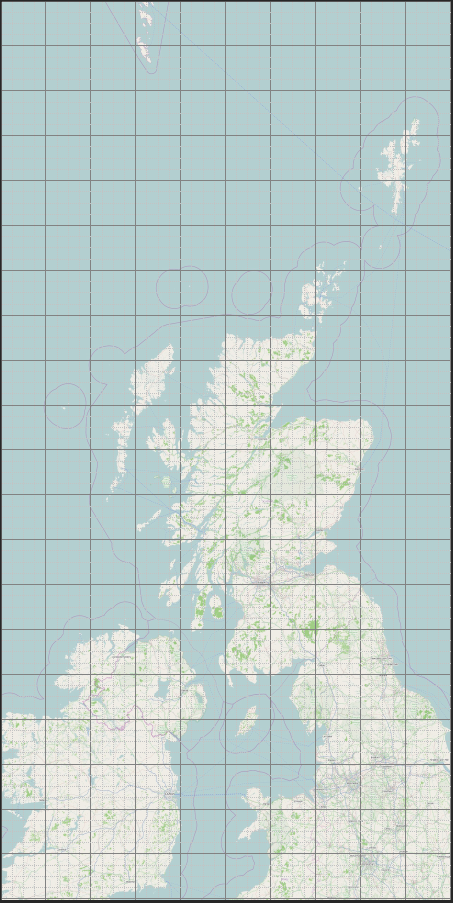
\includegraphics[width=12cm]{./picture/1_1.png}}
  \caption{Total hives of each county in Washington}\label{1_1}
\end{figure}

\begin{figure}[H]
  \centering{
  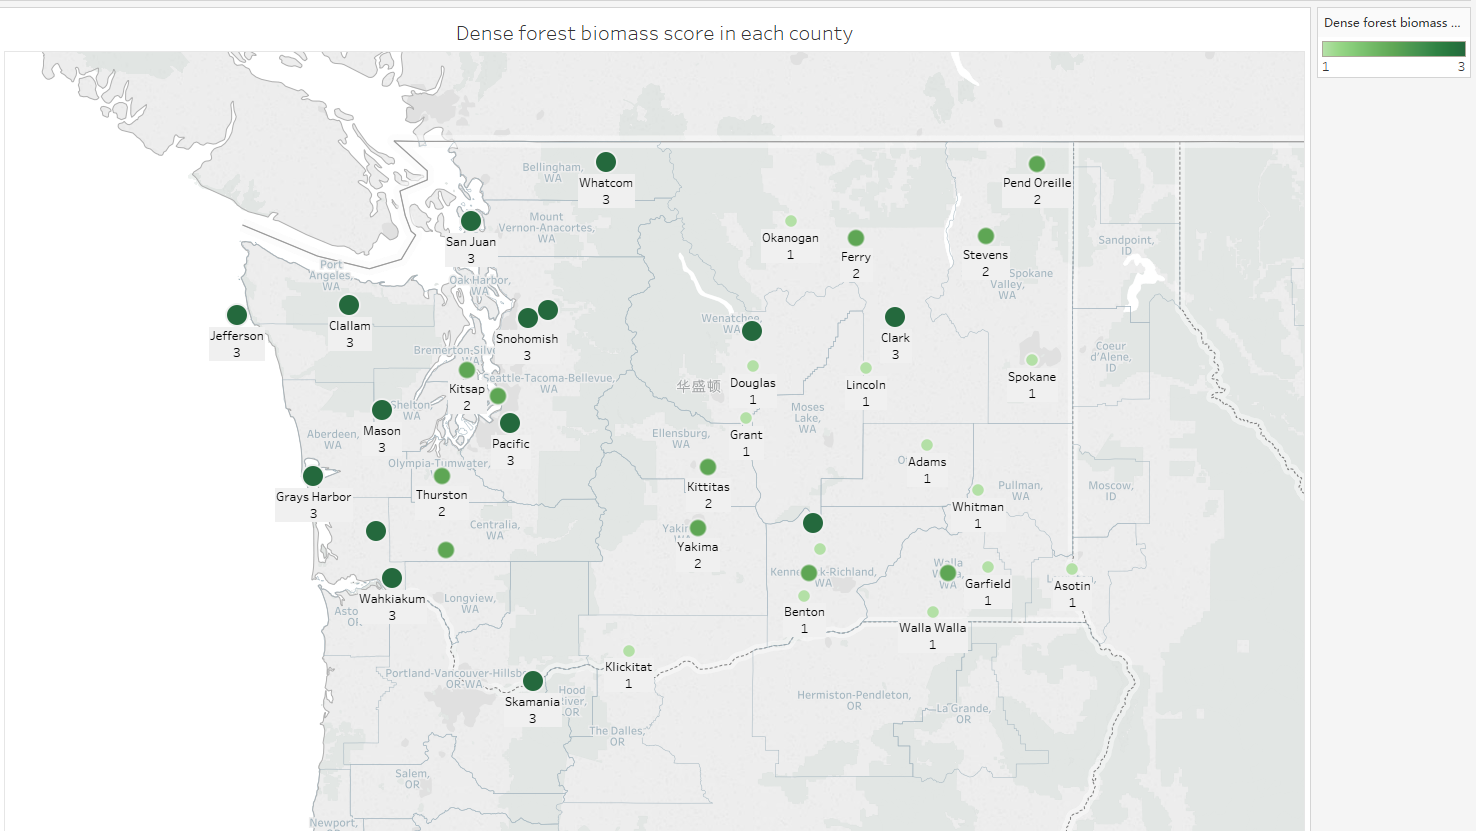
\includegraphics[width=12cm]{./picture/1_2.png}}
  \caption{The dense forest biomass score of each county in Washington}\label{1_2}
\end{figure}

From the above two pictures, we can check the number of hives and the level of vegetation coverage in each county. In addition, we need to consider the county’s transportation convenience level and winter climate comfort. After considering these standards, we will sum up the scores in these four categories and the final score obtained is the risk grade score of the county (appendix quoted table). So far, we can give a risk score to each location in Washington State, and the score only depends on the above four criteria for that location. We denote the risk score of the location of latitude $x$ degrees and longitude $y$ degrees as $F_1(x,y)$.

We combined the above analysis to discuss the distribution of Asian giant hornet over time. We collected information about 14 samples of Asian giant hornet sightings from the official website of the Washington Department of Agriculture (cited), and began to analyze the relevance of the samples. First of all, most of the sighting reports received by the government are not the Asian giant Hornet. We can easily find that the emergence of the Asian Hornet is controlled in a very small area. This may be attributed to the timely and effective measures taken by the government. Secondly, analyzing the time of sightings of the Asian giant Hornet, we can roughly find several earlier positions of the Asian giant Hornet, all of which were before June 2020. The four sighting samples are :
% make a table
\begin{figure}[H]
  \centering
  \subfigure[After 10 years]{               %小图题的名称
  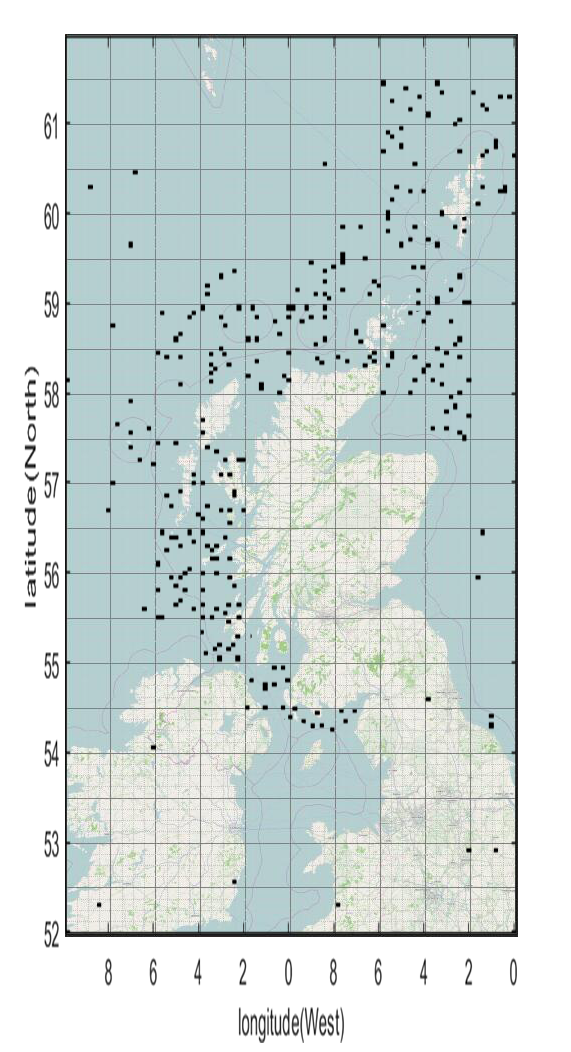
\includegraphics[width=4cm]{./picture/1_10.png}}
  \hspace{0in}
  \subfigure[After 20 years]{
  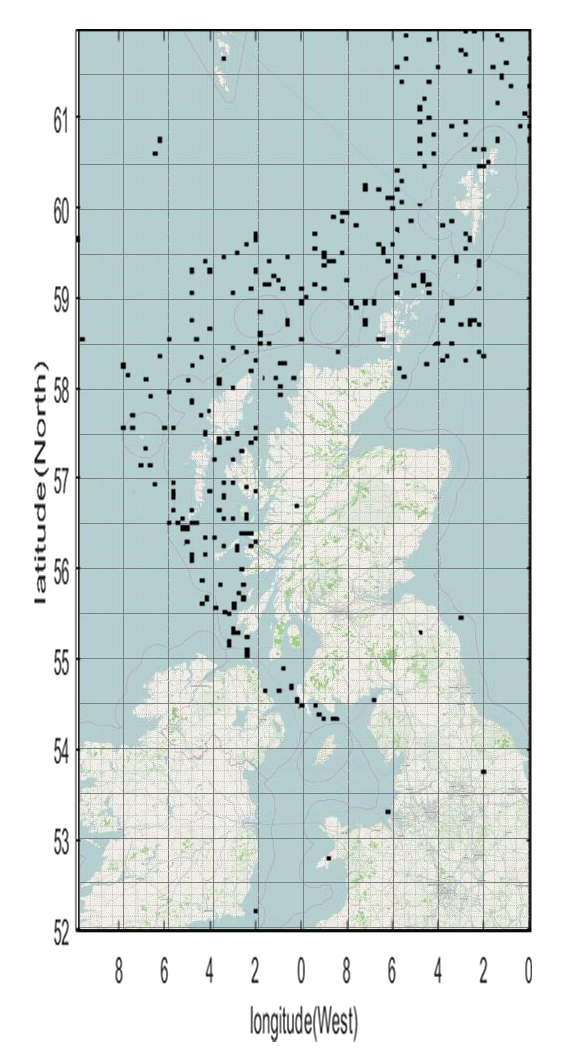
\includegraphics[width=4cm]{./picture/1_11.png}}
  \hspace{0in}
  \subfigure[After 30 years]{
  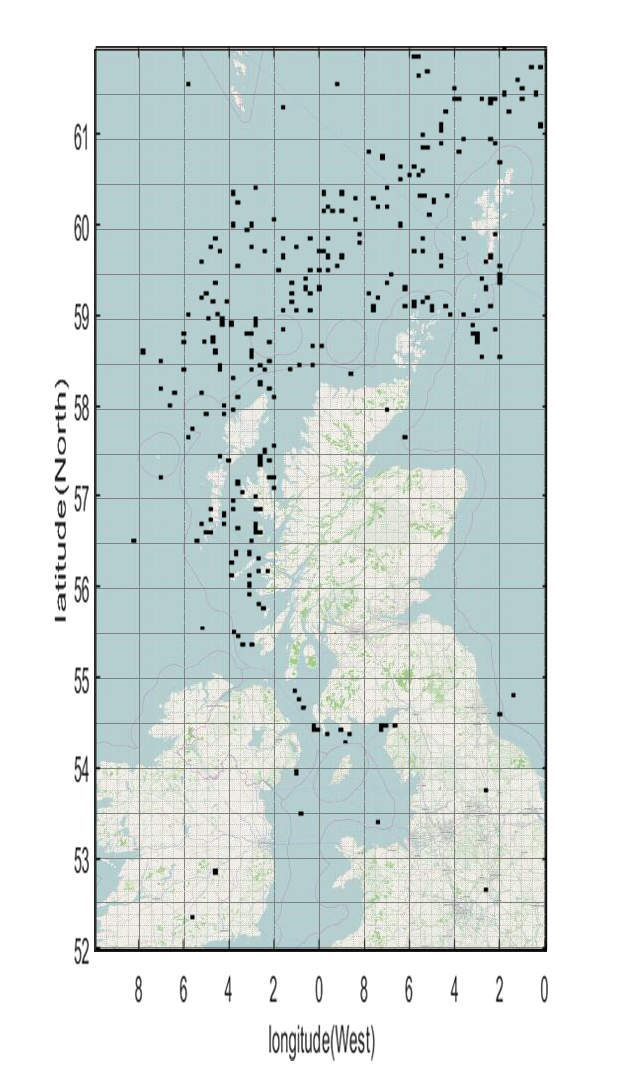
\includegraphics[width=4.2cm]{./picture/1_12.png}}
  \hspace{0in}
  \subfigure[After 40 years]{
  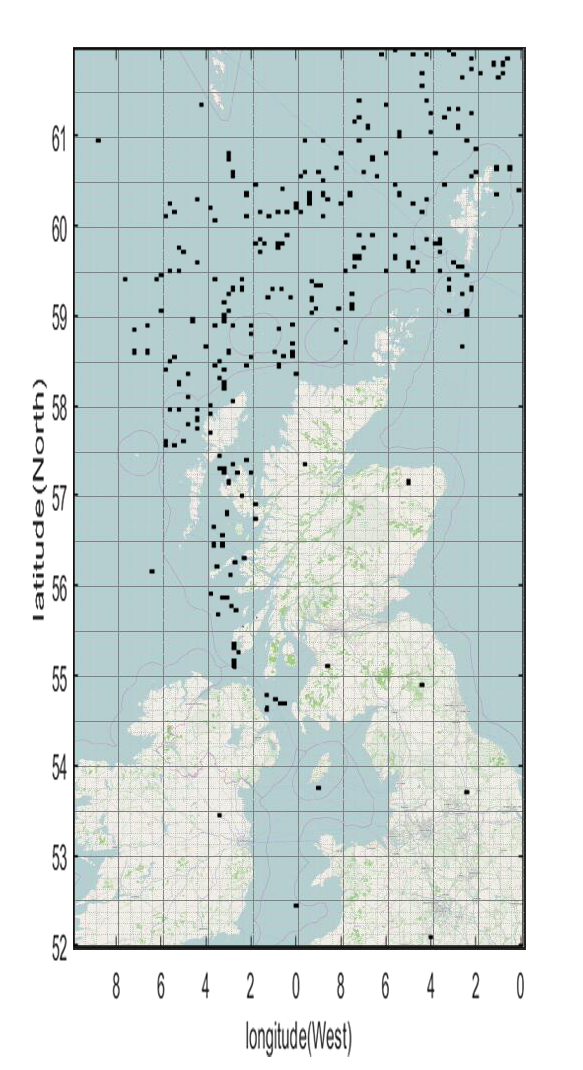
\includegraphics[width=4cm]{./picture/1_13.png}}
  \hspace{0in}
  \subfigure[After 50 years]{
  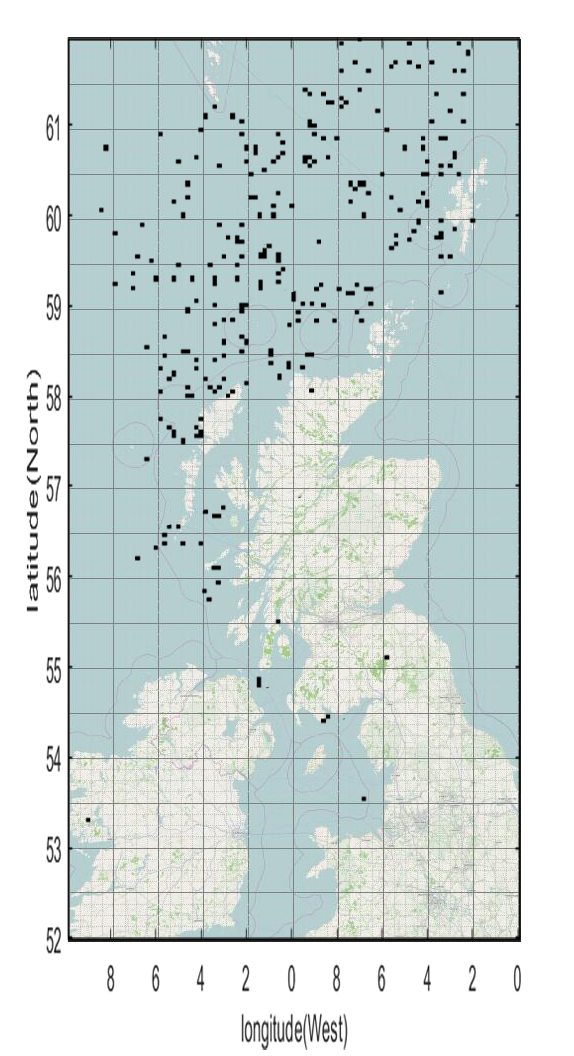
\includegraphics[width=4cm]{./picture/1_14.png}}
  \label{Dist}
  \caption{The prediction of future fish school distribution around Scotland}
  \end{figure}


\begin{figure}[H]
  \centering{
  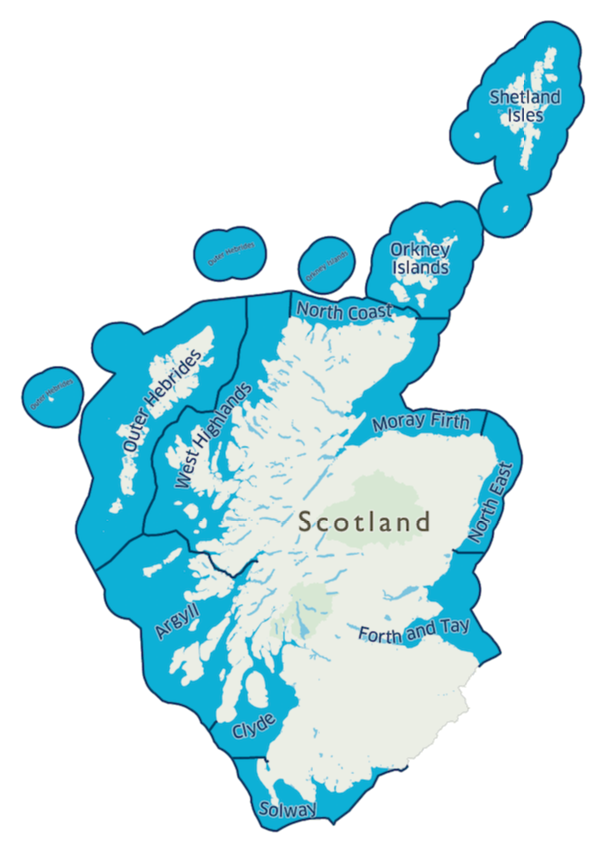
\includegraphics[width=3cm]{./picture/1_3_1.png}}
  \caption{Fisheries around Scotland}\label{FisheriesAround}
\end{figure}

\begin{table}[H]
\centering
\begin{tabular}{|l|l|}% 通过添加 | 来表示是否需要绘制竖线
\hline  % 在表格最上方绘制横线
\textbf{Fishery Name}&\textbf{Representative Color}\\
\hline  %在第一行和第二行之间绘制横线
Argyll \& Clyde & Brown\\
\hline % 在表格最下方绘制横线
Orkney Islands & Yellow\\
\hline % 在表格最下方绘制横线
Outer Hebrides  & Purple\\
\hline % 在表格最下方绘制横线
Shetland Isles & Blue\\
\hline % 在表格最下方绘制横线
North Coast \& West Highlands & Green\\
\hline % 在表格最下方绘制横线
\end{tabular}
\caption{Represntive Color of Fisheries}
\label{FisheryColor}
\end{table}

Then we analyzed the neighborhood relationship between the sighting lFocations of the Asian giant Hornet and found that in the north of San Juan County and in the  of west of Whatcom County, a circular key area was formed. This area is obviously a dense area for Asian giant Hornet sightings. The sighting time of the Asian giant Hornet is probably from September to November 2020. In order to facilitate subsequent processing, we simplify the area to a circle with a radius of $r_0$. Finally, we analyzed the possible migration paths of the Asian giant Hornet. Considering that the road transportation in the key area is more convenient and close to the sea, we infer that the scattered Asian Hornet sightings around the key area may have migrated from the key area. The analysis process of the distribution changes of the Vespa mandarinia over time can refer to the following figure.



\begin{figure}[H]
  \centering{
  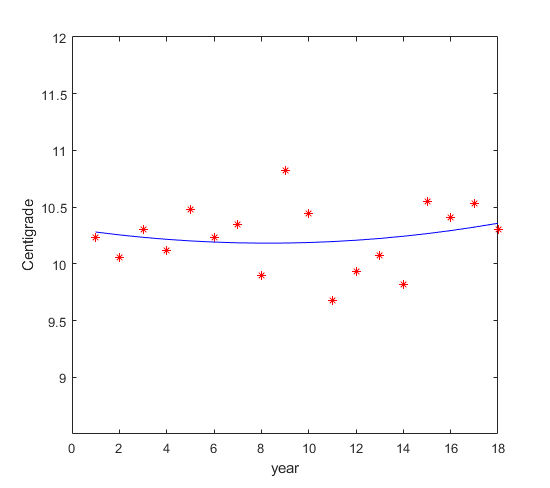
\includegraphics[width=10cm]{./picture/1_4.png}}
  \caption{Schematic diagram of the direction of the Asian Hornet}\label{1_4}
\end{figure}

The blue areas are the earlier areas, but the Asian giant Hornet samples in two blue areas were cleared at the beginning. The red circular area at the border of  Washington State and Canada is the key area with the most reports of Asian giant Hornet sightings. The three black arrows indicate the possible migration routes of Asian giant hornet. The scattered reports may have been migrated by Asian giant hornet in the key area. 

The accuracy of the model can be measured by analyzing the number of positive samples that fall in the key area. We can easily observe that there are 10 points that fall in the red circular area in the above figure. These 10 points occupy more than half of all 18 red points. Our model can accurately reflect the migration trend of Vespa mandarinia.

\subsection{Sighting Report Priority Assessment Model}
\subsubsection{A risk assessment model based on the location of the sighting}
In the above distribution model over time, we can see that sighting location do help us determine the risk rating of the report. Next we will specifically explain the risk assessment model based on the reported sighting location. We believe that the score of this sub-model is a weighted score of the distance to the key area and the risk rating score of the county. In order to simplify the processing, we use the following formula to express:

\begin{equation}
    S_{A(x,y)} = \gamma F_{1(x,y)}+ (1-\gamma) F_{2(x,y)}
\end{equation}

The score of model A at position (x, y) should be weighted by F1 score and F2 score according to the coefficient gamma. 

Among them, F1 is calculated from the distance from the sighting position to the key area, and the calculation formula is as follows:

\begin{equation}
  F_1 = \begin{cases}
    1 & (x-x_0)^2 + (y - y_0)^2 \leq r_{0}^2 \\
    \frac{r_{0}^2}{(x-x_0)^2+(y-y_0)^2} & (x-x_0)^2 + (y-y_0)^2 > r_{0}^2

  \end{cases}
\end{equation}

We simplify the key area to be a circle with $(x_0, y_0)$ as the center and $r_0$ as the radius. The cluster center of Asian giant hornet appearance address is $(x_0, y_0)=(48.99385, -122.6933)$, the radius of the circle $r_0=0.16822856475640974$. When the sighting location  $(x, y)$ falls within the circular area, the value of $F_1$ is 1, which represents the highest risk at this time; when the sighting location $(x, y)$ falls outside the circular area, $F_1$ is an inverse proportional function between the value and the distance. 

The $F_2$ score is determined by the county's risk rating score. In the distribution change model of the Asian giant Hornet, we have checked the number of hives and vegetation coverage in each county, and scored the risk for each county. Therefore, we can directly find the risk score of the county where $(x,y)$ is located, and use it as the $F_2$ score. 

Now for any witness’s report, we can enter the witness location to get the score of the risk assessment model directly, and it will be fused with the following two sub-models.

\subsubsection{A Plain Bayesian-based Review Classification Model}

According to the existing notes, we can see that all reports that were finally identified as positive do not have a specific description of the appearance, while many of the cases of negative and unverified have detailed description about pests. We can conclude that notes are not significant for whether the sighting is an Asian giant Hornet or not, so the notes classification model based on Naive Bayes has the lowest proportion in the fusion model. But it's not saying that these notes are worthless. In negative reports, the most frequently appearing words are often the Asian giant Hornet characteristics that are most misleading. Therefore, based on this, we can use the frequency of high-frequency misleading words to reversely evaluate the probability that witnesses misjudge the Asian giant Hornet report.

\subsubsection{A Plain Bayesian-based Review Classification Model}
According to the existing notes, we can see that all reports that were finally identified as positive do not have a specific description of the appearance, while many of the cases of negative and unverified have detailed description about pests. We can conclude that notes are not significant for whether the sighting is an Asian giant Hornet or not, so the notes classification model based on Naive Bayes has the lowest proportion in the fusion model. But it's not saying that these notes are worthless. In negative reports, the most frequently appearing words are often the Asian giant Hornet characteristics that are most misleading. Therefore, based on this, we can use the frequency of high-frequency misleading words to reversely evaluate the probability that witnesses misjudge the Asian giant Hornet report.

First, we remove the staying words and count the frequency of keywords in all notes. The statistical results can show the corresponding high-frequency words. The statistical results are shown in the following figure:

\begin{figure}[H]
  \centering{
  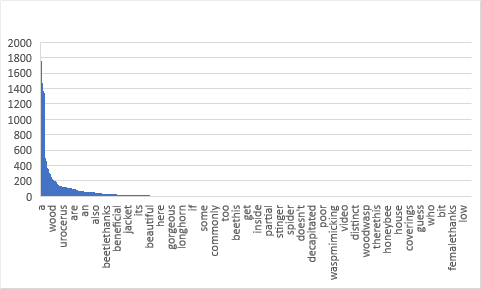
\includegraphics[width=10cm]{./picture/2_1.png}}
  \caption{Sorting of high frequency words in "Negative ID"}\label{sohfw}
\end{figure}

We can see that the first few high-frequency vocabulary are words that people must use in oral speech or words that are not related to Vespa mandarinia. This is a part of vocabulary that are not meaningful, so we remove it. At the same time, in order to reduce the parameters, words that appear less than five times are also removed, and the remaining high-frequency words are sorted as shown in the following figure.

\begin{figure}[H]
  \centering{
  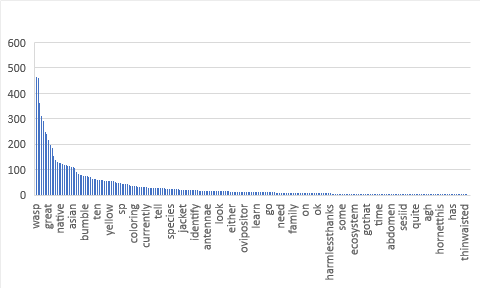
\includegraphics[width=10cm]{./picture/2_2.png}}
  \caption{Sorting of high frequency words in "Negative ID" after filtering}\label{sohfwaf}
\end{figure}

After that, we will use the Naive Bayes algorithm to evaluate the misleadingness of the notes, so as to convert the problem into a classification problem for notes in the report. The reason why we use Naive Bayes is its stable classification efficiency. It performs well on small-scale data, can handle multiple classification tasks, and is suitable for incremental training. And it is not very sensitive to missing data and is relatively simple and often used for text classification.

We assume that the appearance of these high-frequency words is independent, because the naive Bayes algorithm requires that each feature be independent of each other. We can calculate the probability of being misled by witnesses under the premise that certain high-frequency vocabulary appears directly based on the conditional probability formula without training the model. Now for any report, if it contains a note, we can get the probability that the report was misled so as to infer the probability that the report does belong to the Asian giant Hornet. If notes are not provided,  this sub-model is set to be the default score 0.5. Considering that notes are dirty, this model will take the smallest part of the weight in the fusion model.

\subsubsection{EfficientNet-based image classification model}

The first we do is to sort out the image data and corresponding tags from the original data. Normal image data can be processed directly. For video files, we need to manually extract a picture containing bees. For other formats, we just discard them. We sorted out 3294 pictures of Negative ID, 14 pictures of Positive ID, and 97 pictures of Unprocessed and Unverified ID. Up to this point, the data set we have constructed still has the problems of inconspicuous picture subjects and uneven distribution of positive and negative samples.

Since there are few (just 14) positive samples, we use image enhancement technology to expand the number of positive samples from 14 to 1,400. The specific techniques include random flip, rotation, brightness, contrast, color saturation, etc. Finally, the final image is scaled to $224 \times 224$, which can be used as the input of the following neural network. The following is a picture after image enhancement:

\begin{figure}[H]
  \centering{
  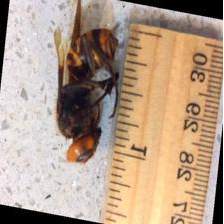
\includegraphics[width=5cm]{./picture/2_3.png}}
  \caption{Picture after image enhancement}\label{sohfwaf}
\end{figure}

Considering that there are only about 100 unlabeled samples, we do not need to adopt a complex semi-supervised learning model, so we only adopt a relatively simple semi-supervised learning method of direct learning. The model assumes that the unlabeled samples are exactly the data to be predicted and only predicts the unlabeled data observed during the learning process, trains these newly labeled unlabeled samples with the previous sample data, and repeats this process until the accuracy of the model no longer improves.

%做表

The processed pictures are fed to neural network training for two classification, and the network output is the probability that the picture belongs to the Asian giant Hornet. After a long period of training, the accuracy of our two-class model reached $96\%$. In order to ensure that the pictures of PositiveID tags are not missed while considering accuracy, we independently verified the recall rate of these 14 pictures, and the model finally classified 13 pictures correctly.

Now for any report, if it contains a picture, we can directly enter the picture to get the score of the picture classification model. If the report does not provide a picture, we default the score of the picture classification model to 0.5. The score of EfficientNet-based picture $S_c(img)$, which will be fused with the other two sub-models and will account for most of the weight.

\subsubsection{The fusion model based on the above three sub-models}

The score of a single model always has limitations, but fusion of the above three sub-models can often improve the robustness of the fusion model. Since each sub-model only focuses on part of the information reported by the witnesses, although this results in a single model that is not so good, but this ensures that these sub-models are independent of each other and there is no correlation between the results, so the effect of the fusion model will be more prominent. Our fusion method uses a relatively simple voting method, and the fusion formula is as follows:

\begin{equation}
  S_{D(x_1 y_2 img,note)} = \alpha S_{A(x,y)}  + \beta S_{B(img)} + (1-\alpha-\beta)S_{c(note)}
\end{equation}

The sub-models A,B and C are weighted and summed according to the ratio of 

%表格
\subsection{Model interpretation and dynamic update}

The output of our model represents the priority processing level of the report. You can see that the highest score is 0.593, so we suggest that if it is higher than the threshold 0.46, then the staff should give priority to processing the report. We believe that when the score of the fusion model is lower than 0.5, the report is most likely to be negative, but for the sake of safety, we recommend that the staffs of the Ministry of Agriculture give priority to all reports with a score greater than 0.46.


\subsection{Model interpretation and dynamic update}

The output of our fusion model represents the priority processing level of the report. If it is higher than the threshold 0.46, the staff should give priority to processing its report. If the reporter provides a picture, then the picture is the best description, and the score of the picture classification model has great reference value. But if the reporter doesn't provide a picture, then according to the neighborhood principle of the distribution of the Asian giant hornet colony, we need to consider the sighting location provided by the witness. Considering that there are too many mixed information in the notes and too many subjective factors, which are not conducive to the objective evaluation of the model, so the priority of notes classification model is the lowest.

As time goes by, the number of reports available for training will gradually increase. In order to ensure that the performance of the fusion model can continue to improve, we need to update the fusion model in a batch learning manner. Specifically, we need to retrain a new version of the system on the basis of new data and old data, and then replace the old system. In order to ensure the timeliness of the model, the weight of the new data should be set larger. After comprehensive consideration, we believe that the condition that triggers the model update should be 400 newly collected reports, and it takes about 20 days to update.

First, we use our model to evaluate the priority of reports with unprocessed and unverified tags. Our default score threshold is 0.5. When the sample score is lower than 0.5, we believe that the bee species corresponding to the report is not an Asian giant Hornet, even if there is a small amount the sample score is slightly greater than 0.5, and we are still confident that the Asian giant Hornet has been eradicated in Washington State under the premise of conforming to the statistical law. The active time of Asian giant hornet is in summer and autumn. The mating season starts in early autumn, and the activity of the colony gradually decreases in late autumn. The queen needs to experience a long overwintering period. Taking these factors into account, as well as the fact that no report of Asian giant hornet has been found for almost three months since mid-November last year, we can speculate that the pest has been eradicated in Washington State.

\section{Model Analysis}
\subsection{Sensitivity Analysis}
Our three sub-models are independent of each other, so fusing them can often improve the robustness of the fusion model. We mentioned earlier that the default weights of these three sub-models are 0.3, 0.1, 0.6, and we will compare different $\alpha$ and $\beta$, hoping to find the best weight ratio.

First, consider our choice of metrics. The classification accuracy of the fusion model is not that important here, because behind the high classification accuracy, the sample recall rate of the positive label may be very low, so that a large number of unimportant samples are likely to be classified correctly, but the most urgent Asian giant Hornet sample is misclassified. Therefore, we believe that the metric should be the recall rate of 14 Asian Hornet samples. The following table is our test results.

% 制表

From the above table, we can see that using our recommended parameter which are $\alpha$=0.3 and $\beta$=0.6, the fusion model has the highest recall rate. Although the recall samples are relatively small and may not reflect the subtle differences of the model, in any case, the EfficientNet model contributes the most to the fusion model. In addition, we can find that model fusion does improve the recall rate of the model to a certain extent, and the strategy of model fusion is successful.

\subsection{Advantages of the model}

\begin{enumerate}
  \item This model comprehensively considers the distribution of bee hives, vegetation coverage, wasp habits and other factors to calculate the risk rating of each county in Washington. And then we establish a multi-modal report priority evaluation model based on the report's notes, pictures and sighting locations. Our fusion model takes a comprehensive consideration of factors and can accurately reflect the priority of reports.
  \item Taking into account the small number of witness notes, the naive Bayes algorithm we use has stable classification efficiency, and performs well on small-scale data, and can be incrementally trained, which is more suitable for this classification task.
  \item We use data enhancement skills to increase the number of positive pictures to increase the robustness and recognition effect of our image recognition model.
  \item We have selected a suitable batch learning period, which can ensure that our model can be continuously optimized with the continuous increase of witness reports, so as to have a better performance effect.
  \item Considering the existence of a large number of unlabeled samples, we use a semi-supervised model method to improve model performance.
\end{enumerate}

\subsection{Disadvantages of the model}
\begin{enumerate}
  \item In the risk assessment model based on sighting locations, our risk assessment based on hive density and vegetation coverage is based on the county as a unit. The measurement scale is too large, which may lead to overestimation or underestimation of actual risks in certain areas.
  \item The notes classification model based on Naive Bayes only calculates the probability that the note is a negative sample based on the statistical results. This is effective in limited notes, but it may make classification result invalid when a new negative note that has not been seen arrives.
  \item In the image classification model based on EfficientNet, although we have increased the number of positive pictures through data enhancement skills, the number of positive pictures is still very small, which will lead to weak generalization or overfitting of the image classification model.
  \item We did not solve the problem that the main body of the Asian giant hornet in the picture is not prominent. For example, the main body of the Asian giant hornet in many pictures is very small, or the Asian giant hornet in the picture is blurred. This problem may reduce the accuracy of the image classification model.
  \item In the image classification model based on EfficientNet, we only deal with image and video formats, and directly discard reports in other formats, which may result in the loss of important emergency reports.
\end{enumerate}

\subsection{Future improvements}

\begin{enumerate}
  \item The risk assessment model based on the sighting location should focus on estimating the risk of a certain area on a more refined scale in the future.
  \item We may build a Knowledge Graph about the Asian giant Hornet based on 2021MCM\_ ProblemC\_ Vespamandarinia.pdf, and then extract the description in the notes to judge the classification based on the knowledge graph. This will greatly improve the accuracy of the notes classification, but it will take a lot of time and energy.
  \item We can obtain more positive pictures through Google Pictures or other databases to improve the generalization ability of the image recognition model.
  \item We can use R-CNN, YOLO or other target detection models to extract the Asian giant Hornet in the image before applying the image classification model, and then use the EfficientNet image classification model to obtain better image recognition results.
  \item We will improve our model by trying more image and text classification baseline models.
  \item We need to spend time programming to automatically extract various format files as pictures.
\end{enumerate}






\newpage
\section{A Summary for the Washington State Department of Agriculture}


Vespa mandarinia has invaded Washington state. This insect tends to destroy bee population and affect human safety due to its bite, which poses a threat to human health and safety of ecosystem, agricultural sector and the areas around their nesting sites. In order to help the Ministry of agriculture eliminate this alien species, we established a model of hornet distribution over time and a priority evaluation model of eyewitness reports. Our fusion model  leads to prioritizing investigation of the reports most likely to be positive sightings.

The life cycle of Vespa mandarinia begins with the nesting of a queen after overwintering. During this period, the queen develops nests, collects and feeds on arthropods and tree sap, and prepares to lay eggs. The colony begins in the summer, the queen takes care of her cubs, and the workers finally begins to appear. Once the queen has enough workers, the responsibility of predation is completely transferred to the workers, while the queen stays in the nest and continues to lay eggs.

Based on the above-mentioned habits of Vespa mandarinia , we studied the population distribution of Vespa mandarinia  over time. After a limited number of samples, we can draw a conclusion that there are three possible migration routes of Vespa mandarinia  and a key area for the emergence of hornets. Because the above conclusions only consider the rules in the real samples of Vespa mandarinia, we also evaluated the bee hive density, vegetation coverage, geography and topography in various counties of Washington state, so as to revise the previous conclusions. As the prey of Vespa mandarinia is mainly bees, and the nesting sites of Vespa mandarinia  are inseparable from vegetation, we should pay more attention to the counties that meet these conditions.

Our model is a fusion model weighted by three sub-models. If the corresponding sub-model has no input data, the default output value is 0.5. Now, according to the pictures provided by the witnesses, the labels of the witnessing insects can be prioritized. If the witnesses do not provide any picture, the position coordinates reported by the witnesses are still of great significance to our investigation. Combined with the distribution of the Asian giant Hornet over time, we can obtain the possibility of finding Asian giant Hornet in the sighting location. If the eyewitness only provides notes, we use the notes classification model to make the final judgment, but the score of this model does not take much weight. There are too much dirty information and too many subjective factors in the notes, which is not conducive to the objective evaluation of the model.

The output of our fusion model represents the priority processing level of the report. If it is higher than the threshold 0.46, the staff should give priority to processing its report. As time goes by, the number of reports available for training will gradually increase. In order to ensure that the performance of the fusion model can continue to improve, we need to update the fusion model in a batch learning manner. We recommend that the condition that triggers the model update should be 400 newly collected reports, and it takes about 20 days to update.

Finally, we evaluated the priority of the reports with unprocessed and unverified labels and found that only a small number of reports scored slightly greater than 0.5. Under the premise of conforming to the laws of statistics, we are confident that the Asian Hornet has been eradicated in Washington State. The activity of the Asian giant hornet gradually decreases in late autumn, and the queen bee needs to experience a long overwintering period. From the information on the official website, we found that no sample of Asian Hornet has been found in the almost three months since mid-November last year. It can be assumed that the pest has been eradicated in Washington State.


\newpage
\addcontentsline{toc}{section}{Reference}
\bibliographystyle{plain}
\bibliography{myreference}



\end{document}
